\documentclass{article}

\usepackage{listings}
\usepackage{fancyhdr}
\usepackage{extramarks}
\usepackage{amsmath}
\usepackage{amsthm}
\usepackage{amsfonts}
\usepackage{tikz}
\usepackage[plain]{algorithm}
\usepackage{algpseudocode}

\usetikzlibrary{automata,positioning}

%
% Basic Document Settings
%

\topmargin=-0.45in
\evensidemargin=0in
\oddsidemargin=0in
\textwidth=6.5in
\textheight=9.0in
\headsep=0.25in

\linespread{1.1}

\pagestyle{fancy}
\lhead{\hmwkAuthorName}
\chead{\hmwkClass\ (\hmwkClassInstructor\ \hmwkClassTime): \hmwkTitle}
\rhead{\firstxmark}
\lfoot{\lastxmark}
\cfoot{\thepage}

\renewcommand\headrulewidth{0.4pt}
\renewcommand\footrulewidth{0.4pt}

\setlength\parindent{0pt}

%
% Create Problem Sections
%

\newcommand{\enterProblemHeader}[1]{
    \nobreak\extramarks{}{Problem \arabic{#1} continued on next page\ldots}\nobreak{}
    \nobreak\extramarks{Problem \arabic{#1} (continued)}{Problem \arabic{#1} continued on next page\ldots}\nobreak{}
}

\newcommand{\exitProblemHeader}[1]{
    \nobreak\extramarks{Problem \arabic{#1} (continued)}{Problem \arabic{#1} continued on next page\ldots}\nobreak{}
    \stepcounter{#1}
    \nobreak\extramarks{Problem \arabic{#1}}{}\nobreak{}
}

\setcounter{secnumdepth}{0}
\newcounter{partCounter}
\newcounter{homeworkProblemCounter}
\setcounter{homeworkProblemCounter}{1}
\nobreak\extramarks{Problem \arabic{homeworkProblemCounter}}{}\nobreak{}

\newenvironment{homeworkProblem}{
    \section{Problem \arabic{homeworkProblemCounter}}
    \setcounter{partCounter}{1}
    \enterProblemHeader{homeworkProblemCounter}
}{
    \exitProblemHeader{homeworkProblemCounter}
}

%
% Homework Details
%   - Title
%   - Due date
%   - Class
%   - Section/Time
%   - Instructor
%   - Author
%

\newcommand{\hmwkTitle}{Homework\ \#9}
\newcommand{\hmwkDueDate}{July 29, 2019}
\newcommand{\hmwkClass}{Introduction to Cryptography}
\newcommand{\hmwkClassTime}{}
\newcommand{\hmwkClassInstructor}{Professor Manuel}
\newcommand{\hmwkAuthorName}{ShiHan Chan}

%
% Title Page
%

\title{
    \vspace{2in}
    \textmd{\textbf{\hmwkClass:\ \hmwkTitle}}\\
    \normalsize\vspace{0.1in}\small{Due\ on\ \hmwkDueDate\ at 11:59pm}\\
    \vspace{0.1in}\large{\textit{\hmwkClassInstructor\ \hmwkClassTime}}
    \vspace{3in}
}

\author{\textbf{\hmwkAuthorName}}
\date{}

\renewcommand{\part}[1]{\textbf{\large Part \Alph{partCounter}}\stepcounter{partCounter}\\}

%
% Various Helper Commands
%

% Useful for algorithms
\newcommand{\alg}[1]{\textsc{\bfseries \footnotesize #1}}

% For derivatives
\newcommand{\deriv}[1]{\frac{\mathrm{d}}{\mathrm{d}x} (#1)}

% For partial derivatives
\newcommand{\pderiv}[2]{\frac{\partial}{\partial #1} (#2)}

% Integral dx
\newcommand{\dx}{\mathrm{d}x}

% Alias for the Solution section header
\newcommand{\solution}{\textbf{\large Solution}}

% Probability commands: Expectation, Variance, Covariance, Bias
\newcommand{\E}{\mathrm{E}}
\newcommand{\Var}{\mathrm{Var}}
\newcommand{\Cov}{\mathrm{Cov}}
\newcommand{\Bias}{\mathrm{Bias}}

\begin{document}

\maketitle

\pagebreak

\begin{homeworkProblem}
We can use (t,w) threshold scheme to solve this problem. Let t=10, w=30. Give each general 10 shares, give each colonel 5 shares, and give each clerk 2 shares.\\
\end{homeworkProblem}

\pagebreak


\begin{homeworkProblem}
Let $2 <= k <= n$ be integers. We generate a sequence of pairwise coprime positive integers $ m_{0}<...<m_{n} m_{0}<...<m_{n}$ such that $m_{0}.m_{n-k+2}...m_{n}<m_{1}...m_{k}$ . For the sequence, the secret S is a random integer in the set Z/m0Z.\\
We pick  a random integer $\alpha$ such that $S+\alpha \cdot m_{0}<m_{1}...m_{k}$. We compute the reduction modulo $m_i$ of $S+\alpha \cdot m_{0}$, for all $1 <= i <= n$, there are shares $I_{i}=(s_{i},m_{i})$. Now, for each k different share $I_{i_{1}},...,I_{i_{k}}$, we find the system of congruences below:
\begin{figure}[h]
	\graphicspath{images}
	\begin{center}
		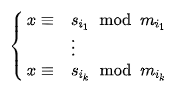
\includegraphics[scale=0.7,command=Figure1: Vigenère cipher]{images/CRT.png}
	\end{center}
\end{figure} 
\\
We use the Chinese remainder theorem to solve the system, since $m_{i_{1}},\ldots ,m_{i_{k}}$ are pairwise coprime, the system has a unique solution modulo $m_{i_{1}}\cdots m_{i_{k}}$. By the construction of our shares, the secret S is recovered.
\\
\end{homeworkProblem}
\pagebreak
\begin{homeworkProblem}
We first define Lagrange basis polynomials as follow:\\
$l_i(x)=\frac{(x-x_0)\cdots(x-x_{i-1})(x-x_{i+1})\cdots(x-x_n)}{(x_i-x_0)\cdots(x_i-x_{i-1})(x_i-x_{i+1})\cdots(x_i-x_n)}$\\
$p(x)=\sum_{i=0}^n y_il_i(x)$\\
When this is applied to the scheme, every value should modulo p. Then $k$ multiple of $\frac{p(x-x_0)\cdots(x-x_{i-1})(x-x_{i+1})\cdots(x-x_n)}{(x_i-x_0)\cdots(x_i-x_{i-1})(x_i-x_{i+1})\cdots(x_i-x_n)}$ 
should be added to each $l_i(x)$ when we reconstruct the polynomial $p(x)$  to make sure each parameter is integer.\\

We use numbers on lecture slide as an example, set $m=190503180520$, $r_1=482943028839$, $r_2=1206749628665$,$p=1234567890133$ we can choose 2, 3 and 7, and we can get:\\

$x_0=2 \quad y_0=1045116192326 $\\
$x_1=3 \quad y_1=154400023692$ \\
$x_2=7 \quad y_2=973441680328$

And we can calculate $l_i$\\

$l_0(x) = \frac{(x-3)(x-7)}{(2-3)(2-7)}=\frac{1}{5}(x-3)(x-7)$ \\
$l_1(x) = \frac{(x-2)(x-7)}{(3-2)(3-7)}=-\frac{1}{4}(x-2)(x-7)$ \\
$l_2(x) = \frac{(x-2)(x-3)}{(7-2)(7-3)}=\frac{1}{20}(x-2)(x-3)$



$p(x) = y_0l_0(x)+y_1l_1(x)+y_2l_2(x)$ \\
$= \frac{1045116192326}{5}(x-3)(x-7)-\frac{154400023692}{4}(x-2)(x-7)+\frac{973441680328}{20}(x-2)(x-3)$ 
$= \frac{1095476582793}{5}x^2-1986192751427x+\frac{20705602144728}{5}$\\
$r_2 \equiv \frac{1095476582793}{5}+\frac{4}{5}p \equiv 1206749628665 \mod p$\\
$r_1 \equiv -1986192751427 \equiv 482943028839 \mod p$\\
$m \equiv \frac{20705602144728}{5}+\frac{4}{5}p \equiv 190503180520 \mod p$\\
\end{homeworkProblem}
\pagebreak
\begin{homeworkProblem}
1.\\
z=2x+3y+13=5x+3y+1\\
12=3x, x=4.\\
So Alice and Bob can recover secret x without the help of Charly.\\
2.\\
We prove this by induction.\\
When $n=2$, $\det V=x_2-x_1=\prod_{1\leq j\leq k\leq 2}(x_k-x_j)$\\
When $n=m\geq 2$, suppose $\det V=\prod_{1\leq j\leq k\leq m}(x_k-x_j)$\\
When $n=m+1$, 
 $\det V=
 \begin{vmatrix}
 1 & x_1 & \cdots & x_1^{m-1} & x_1^m \\
 1 & x_2 & \cdots & x_2^{m-1} & x_2^m \\
 \vdots & \vdots & \ddots & \vdots & \vdots \\
 1 & x_m & \cdots & x_m^{m-1} & x_m^m \\
 1 & x_{m+1}^2 & \cdots & x_{m+1}^{m-1} & x_{m+1}^m \\
 \end{vmatrix}
 $
 \\
 Start from the last column to the second column, we mutiply the left column of current column by $-x_{m+1}$ and it to current column, then we can get:\\
 $
 \det V=
 \begin{vmatrix}
 1 & x_1-x_{m+1} & \cdots & x_1^{m-2}(x_1-x_{m+1}) & x_1^{m-1}(x_1-x_{m+1}) \\
 1 & x_2-x_{m+1} & \cdots & x_2^{m-2}(x_2-x_{m+1}) & x_2^{m-1}(x_2-x_{m+1}) \\
 \vdots & \vdots & \ddots & \vdots & \vdots \\
 1 & x_m-x_{m+1} & \cdots & x_m^{m-2}(x_m-x_{m+1}) & x_m^{m-1}(x_2-x_{m+1}) \\
 1 & 0 & \cdots & 0 & 0 \\
 \end{vmatrix}\\
 =\prod_{i=1}^m(x_{m+1}-x_i)
 \begin{vmatrix}
 1 & x_1 & \cdots & x_1^{m-2} & x_1^{m-1} \\
 1 & x_2 & \cdots & x_2^{m-2} & x_2^{m-1} \\
 \vdots & \vdots & \ddots & \vdots & \vdots \\
 1 & x_{m-1} & \cdots & x_{m-1}^{m-2} & x_{m-1}^{m-1} \\
 1 & x_m^2 & \cdots & x_m^{m-2} & x_m^{m-1} \\
 \end{vmatrix}\\
 =\prod_{i=1}^m(x_{m+1}-x_i)\det V\\
 =\prod_{i=1}^m(x_{m+1}-x_i)\prod_{1\leq j\leq k\leq m}(x_k-x_j)\\
 =\prod_{1\leq j\leq k\leq m+1}(x_k-x_j)
$\\
So we finish to prove this by induction.\\
\end{homeworkProblem}
\pagebreak
\begin{homeworkProblem}
1.\\
Given a finite field F and F[X] is the set of polynomials. n,k are parameters such that $1\leq k\leq n\leq |F|$. Choose n elements from F and form the set {$x_1,x_2,x_3,x_4......x_n$}, and we calculate $C={(f(x_1),f(x_2),..., f(x_n))|f\in F[X],deg(f)<k}$. C is [n,k,n+k-1] code. In the other word, the length is n, the degree is k, smallest distance is n-k+1 code. And $n=|F|-1$.
\\
2.\\
Because any two different polynomials of degree smaller or equal than k-1 intersect in at most k-1 points, this implies that any two codewords of the Reed Solomon code disagree in at least n-(k-1)=n-k+1 points. So the distance of the Reed-Solomon code is n−k+1.
By theorem on slide, we know it is possible to identify a parent of a descendant of $C\subset (F_q)^n$ if $D>n(1- \frac{1}{w^2})$\\
When w = 2, $n-k+1>\frac{3n}{4}$\\
And we can get: $n > 4k-4$\\
\end{homeworkProblem}

\end{document}
